% Pandoc template for Physical Review D (REVTeX 4.2, preprint/one-column).
% Engine: pdflatex — REVTeX is pdflatex-native; xelatex+STIX lacks the glyph REVTeX
% uses for the email footnote marker. Prose Unicode is handled by newunicodechar below.
\documentclass[aps,prd,preprint,nofootinbib,superscriptaddress]{revtex4-2}
\usepackage{iftex}
\ifPDFTeX
  \usepackage[T1]{fontenc}
  \usepackage[utf8]{inputenc}
\else
  \usepackage{fontspec}
  \setmainfont{STIX Two Text}
\fi

\usepackage{amsmath,amssymb,graphicx}
\usepackage[hidelinks]{hyperref}
\usepackage{orcidlink}

% make bare math commands the preprocessors may leave in text mode robust (surd etc.)
\makeatletter
\let\pandocsurd\surd \renewcommand{\surd}{\ensuremath{\pandocsurd}}
\makeatother

% --- prose Unicode operators -> math (works under xe/pdf latex) ---
\usepackage{newunicodechar}
\newunicodechar{→}{\ensuremath{\rightarrow}}
\newunicodechar{∂}{\ensuremath{\partial}}
\newunicodechar{∈}{\ensuremath{\in}}
\newunicodechar{∎}{\ensuremath{\blacksquare}}
\newunicodechar{□}{\ensuremath{\Box}}
\newunicodechar{∝}{\ensuremath{\propto}}
\newunicodechar{∞}{\ensuremath{\infty}}
\newunicodechar{∫}{\ensuremath{\int}}
\newunicodechar{≈}{\ensuremath{\approx}}
\newunicodechar{≠}{\ensuremath{\neq}}
\newunicodechar{≡}{\ensuremath{\equiv}}
\newunicodechar{≤}{\ensuremath{\leq}}
\newunicodechar{≥}{\ensuremath{\geq}}
\newunicodechar{≪}{\ensuremath{\ll}}
\newunicodechar{≫}{\ensuremath{\gg}}
\newunicodechar{≲}{\ensuremath{\lesssim}}
\newunicodechar{⊙}{\ensuremath{\odot}}
\newunicodechar{⊗}{\ensuremath{\otimes}}
\newunicodechar{⟹}{\ensuremath{\Longrightarrow}}
\newunicodechar{⟺}{\ensuremath{\Longleftrightarrow}}
\newunicodechar{⇒}{\ensuremath{\Rightarrow}}
\newunicodechar{⇔}{\ensuremath{\Leftrightarrow}}
\newunicodechar{𝓗}{\ensuremath{\mathcal{H}}}
\newunicodechar{√}{\ensuremath{\surd}}
\newunicodechar{∼}{\ensuremath{\sim}}
\newunicodechar{∇}{\ensuremath{\nabla}}
\newunicodechar{↔}{\ensuremath{\leftrightarrow}}
\newunicodechar{⟨}{\ensuremath{\langle}}
\newunicodechar{⟩}{\ensuremath{\rangle}}
\newunicodechar{−}{\ensuremath{-}}
\newunicodechar{ℓ}{\ensuremath{\ell}}
\newunicodechar{ħ}{\ensuremath{\hbar}}
\newunicodechar{′}{\ensuremath{{}^\prime}}
\newunicodechar{Ḣ}{\ensuremath{\dot H}}
\newunicodechar{Ṡ}{\ensuremath{\dot S}}
\newunicodechar{₊}{\ensuremath{{}_{+}}}

% --- pandoc body requirements ---
\usepackage{longtable,booktabs,array}
\usepackage{calc}
\usepackage{float}
\makeatletter
\newsavebox\pandoc@box
\newcommand*\pandocbounded[1]{%
  \sbox\pandoc@box{#1}%
  \Gscale@div\@tempa{\textheight}{\dimexpr\ht\pandoc@box+\dp\pandoc@box\relax}%
  \Gscale@div\@tempb{\linewidth}{\wd\pandoc@box}%
  \ifdim\@tempb\p@<\@tempa\p@\let\@tempa\@tempb\fi%
  \ifdim\@tempa\p@<\p@\scalebox{\@tempa}{\usebox\pandoc@box}%
  \else\usebox{\pandoc@box}%
  \fi%
}
\makeatother
\providecommand{\tightlist}{\setlength{\itemsep}{0pt}\setlength{\parskip}{0pt}}
\graphicspath{{../}{../figures/}}

\setlength{\emergencystretch}{3em}

\begin{document}

\title{Entropy-Clock Counter-rotating Co-genesis: Baryons and
\textasciitilde1.78 GeV Asymmetric Dark Matter from Pre-inflationary
Initial Conditions}

\author{Stilian Pandev\,\orcidlink{0009-0005-8153-071X}}
\email{stilianpandev@gmail.com}
\affiliation{Independent researcher}

\begin{abstract}
We present a mechanism in which the baryon asymmetry and dark matter
share a single origin fixed by \emph{pre-inflationary initial
conditions} rather than thermal freeze-out. Two counter-rotating hidden
condensates carry a \(\mathrm{U}(1)_{\mathcal{Q}}\) charge with equal
and opposite sign --- we postulate \(Q_V = -Q_D\) --- so that the
comoving \emph{difference} charge \(a^{3}(n_V - n_D)\) is exactly
conserved and the visible and dark sectors leave a first-order, CP-odd
transition at a nucleation temperature \(T_n \approx 3.2\times10^{12}\)
GeV with equal-and-opposite chemical potentials. This
\emph{counter-rotating co-genesis} (ECCG) sits in the Affleck--Dine /
asymmetric-dark-matter (ADM) class
\citep{Kaplan:2009ag, Petraki:2013wwa, Zurek:2013wia, Cheung:2011if}
with a darkogenesis-style first-order impulse
\citep{Shelton:2010ta, Hall:2019rld} --- not a new mechanism
\emph{class} --- but the architecture is specific and makes a sharp,
falsifiable commitment: \textbf{dark matter is \emph{asymmetric} and
light, \(m_X \approx 1.78\) GeV}, a GeV-scale direct-detection and
collider target, so the model is excluded if dark matter is established
as symmetric/thermal or far from the GeV window. Throughout, we are
explicit about which statements are calculated here, which are fixed by
matching data, and which are postulated, assumed, constructed, or
preliminary. Standard-Model sphaleron reprocessing transfers a fixed
fraction \(f_B = 28/79\) \citep{Harvey:1990qw} of the \(B{-}L\)
asymmetry into baryons; we show this textbook value carries over to ECCG
because the dark sector is Standard-Model-singlet and chemically
decoupled at the electroweak scale
(\(\Gamma_{\rm mix}/H = 7.5\times10^{-4}\)), making \(f_B = 28/79\) the
one genuinely calculated closure of the mechanism --- argued (not
re-derived operator-by-operator) to carry over unmodified. The shared
asymmetry then fixes
\(m_X = (\Omega_X/\Omega_b)\, m_p\,(28/79) \approx 1.78\) GeV by
matching the observed \(\Omega_{\rm DM}/\Omega_b\) (matched, not
predicted independently). A distinct realization --- ``Candidate C'' ---
ties \(\eta_B \propto T_{\rm RH}^{2}\,(\Sigma m_\nu)^{2}\) to neutrino
masses; hybridized with ECCG's reheating window it squeezes to
\textbf{normal ordering, \(\Sigma m_\nu \approx 59\text{–}64\) meV, and
\(T_{\rm RH} \approx 3.3\times10^{12}\) GeV} \citep{Elbers:2025vlz}. We
are explicit that this range \emph{brushes the normal-ordering floor}
(\(\Sigma m_\nu \gtrsim 58\) meV): it is a \textbf{consistency
constraint, not a discriminating prediction} --- its confirmation would
not single out ECCG, and its inverted-ordering falsification is DESI's
own conclusion, independent of this model. It survives in only
\textasciitilde1\% of prior impulse-volume, so it constrains the
mechanism without testing it against the null. The magnitude of
\(\eta_B\) is irreducibly a fit; the microscopic strong-coupling inputs
(the first-order transition, the confining vacuum, the wall velocity)
are validated pipelines producing preliminary numbers, not confirmed
results. We say so throughout, and list the falsifiers.
\end{abstract}

\maketitle

\noindent\textbf{Keywords:} baryogenesis; asymmetric dark matter;
co-genesis; first-order phase transition; hidden sector; CP violation
\vspace{6pt}

\section{Introduction}\label{sec-1}

Two of cosmology's stubborn number problems are the baryon asymmetry
\(\eta_B \equiv n_B/n_\gamma = 6.1\times10^{-10}\) and the dark-matter
density \(\Omega_{\rm DM} h^{2} \approx 0.12\), with the further nagging
fact that \(\Omega_{\rm DM}/\Omega_b \approx 5\) is an
\emph{order-unity} ratio rather than the many-decade gap one would
naively expect from unrelated sectors
\citep{Boucenna:2013wba, Davoudiasl:2012uw}. Asymmetric dark matter
(ADM) frameworks \citep{Kaplan:2009ag, Petraki:2013wwa, Zurek:2013wia}
explain the coincidence by sourcing both sectors from one asymmetry; the
price is usually a new mechanism to communicate it. This paper is the
matter-genesis face of a larger program --- the Unified
Structural-Entropy Cosmogenesis (USC) --- which posits a single
horizon-entropy ``clock'' \(\mathcal{D}_E = (3/2)(1-w)\) joining three
physical faces: \textbf{dusk} (dark energy without \(\Lambda\); {[}Paper
III / SEDE cosmology, Zenodo 10.5281/zenodo.21525525{]}), \textbf{dawn}
(this paper), and \textbf{galactic} (a MOND readout; Paper VIII / APDM
galactic, Zenodo 10.5281/zenodo.21525537). The scale sector {[}Paper VI
/ scale sector, Zenodo 10.5281/zenodo.21525533{]} sets the mass scales
that this paper's dark-matter horns draw on. The full unification is
formalized in the umbrella paper {[}Paper V / USC framework{]}, and
every paper cites the frozen pre-registration falsifier matrix (Zenodo
\texttt{10.\allowbreak 5281/\allowbreak zenodo.\allowbreak 21415326}).

The dawn mechanism, ECCG (Entropy-Clock Counter-rotating Co-Genesis),
works as follows. A hidden gauge sector \(\mathrm{SU}(3)_H\) supports
two condensates carrying opposite \(\mathrm{U}(1)_{\mathcal{Q}}\)
charges (\(Q_V = -Q_D\)). A first-order transition in the early universe
gives these condensates a CP-odd impulse; the equal-and-opposite charge
structure means the visible and dark sectors leave the transition with
equal-and-opposite chemical potentials. The Standard-Model electroweak
sphaleron then converts a calculable fraction of the resulting \(B{-}L\)
into baryon number, and the leftover dark charge freezes out as
asymmetric dark matter whose \emph{mass is fixed by the shared
asymmetry} --- the ADM co-genesis logic in its cleanest form
\citep{March-Russell:2011ang, Cheung:2013dca}. The counter-rotating
condensate architecture --- a charge carried with equal-and-opposite
sign in the visible and dark sectors, so that a comoving asymmetry is
conserved and the two sectors inherit opposite chemical potentials ---
is closest in spirit to Affleck-Dine cogenesis \citep{Cheung:2011if};
the hidden first-order-transition route from which the impulse is
sourced parallels darkogenesis \citep{Shelton:2010ta} and asymmetric
matter from a dark first-order phase transition \citep{Hall:2019rld}.

We are deliberately austere about what this buys. ECCG is best described
as a \textbf{matched-EFT existence proof} of GeV-scale asymmetric
co-genesis with one sharp handle (\(m_X \approx 1.78\) GeV), not a fully
predictive theory: the \emph{sign} of the asymmetry is environmental,
the \emph{magnitude} of \(\eta_B\) is a fit, and the microscopic
strong-coupling inputs are benchmark-grade. The value of the
construction is (i) the single genuinely-calculated closure
(\(f_B = 28/79\)), (ii) the near-floor neutrino \emph{consistency
constraint} of the Candidate-C variant, and (iii) the way the dawn face
over-determines itself against the rest of the program through the
shared clock and the identity \(\omega_b \equiv \eta_B\).

\subsection{The connection to the entropy clock --- and an important
negative result}\label{sec-1-1}

The wider program is organized around an entropy clock
\(\Theta_E = \ln(3H/4Gs)\), \(\mathcal{D}_E = (3/2)(1-w)\), which reads
\(\mathcal{D}_E \approx 1\) at the dawn (radiation-like) and
\(\mathcal{D}_E \to 3\) at the dusk (de Sitter-like). It is tempting ---
and the early ECCG development attempted this --- to have the clock
\emph{directly source} the matter asymmetry through a
spontaneous-baryogenesis chemical potential \(\mu_Q/T \propto H/T\).
\textbf{That direct-source mechanism is dead} (a calculated, proven
negative): the arrow operator that would source it is
\(\mathbb{Z}_2\)-even, so its coefficient \(R_0 = 0\) by symmetry, and
independent yield estimates fall short by many orders of magnitude. We
state this plainly because it is load-bearing for the program's honesty:
\emph{the clock does not source matter.} ECCG is a
\textbf{pre-inflationary initial-condition theory} --- the asymmetry is
laid down by the condensate impulse at a first-order transition, not
pumped by the clock --- and the clock's role in the dawn is confined to
the timing/thermodynamic backdrop and the over-determination
bookkeeping. The \(R_0 = 0\) no-go is what forced the program to this
honest, narrower position.

\begin{center}\rule{0.5\linewidth}{0.5pt}\end{center}

\section{The mechanism}\label{sec-2}

\begin{figure}
\centering
\pandocbounded{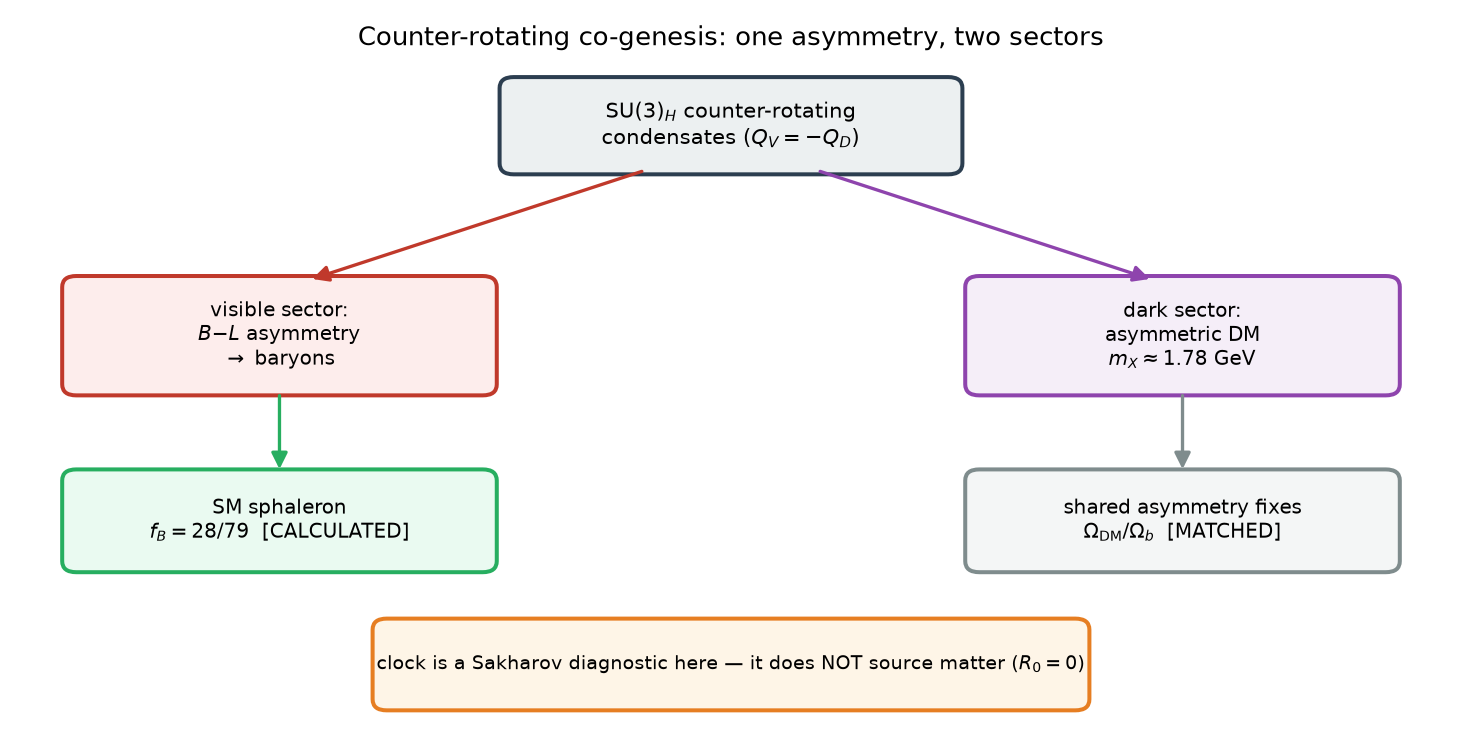
\includegraphics[keepaspectratio]{figures/fig1_mechanism.png}}
\caption{Counter-rotating co-genesis. SU(3)\(_H\) counter-rotating
condensates (\(Q_V=-Q_D\)) seed a \(B{-}L\) asymmetry that the SM
sphaleron transfers to baryons with the calculated fraction
\(f_B=28/79\), and a shared asymmetry in the dark sector fixing an
asymmetric dark-matter density (\(m_X\approx1.78\) GeV,
\(\Omega_{\rm DM}/\Omega_b\) matched). The entropy clock is a Sakharov
diagnostic here --- by the \(R_0=0\) theorem it does not itself source
matter.}\label{fig:1}
\end{figure}

\subsection{Counter-rotating condensates and the conserved comoving
asymmetry}\label{sec-2-1}

The field content of the ECCG benchmark comprises a hidden
\(\mathrm{SU}(3)_H\) gauge sector, a \(\mathbb{Z}_{31}\) flavor
structure, a \(\mathrm{U}(1)_{\mathcal{Q}}\) under which two scalar
condensates \(\Phi_V, \Phi_D\) carry \textbf{equal and opposite charge}
\(Q_V = -Q_D\), which we postulate as the defining structural assumption
of the model. The immediate consequence is a conservation law,

\begin{quote}
\(d/dt\,[\,a^{3}\,(n_V - n_D)\,] = 0\), i.e.~\(Q_V = -Q_D \Rightarrow\)
a conserved comoving \emph{difference} charge (calculated, given the
charge assignment).
\end{quote}

Two independent ECCG codebases converge on this equal-and-opposite
structure, the transfer ratio \(R_{\rm tr}\), and \(m_X\)
(\texttt{CROSS\_\allowbreak CHECK\_\allowbreak MEMO.\allowbreak md}: ``AGREE''; \(m_X = 1.33\) vs \(1.3255\)
GeV in the older flavored normalization). The counter-rotating structure
is what makes this a \emph{co-genesis}: the same impulse that populates
the visible \(B{-}L\) populates the dark charge, with a fixed relative
sign, so the two abundances are locked together. This conserved
counter-rotating charge structure --- equal-and-opposite \(Q_V = -Q_D\)
with a conserved comoving difference \(a^{3}(n_V - n_D)\) and
equal-and-opposite chemical potentials --- is the closest prior art to
Affleck-Dine cogenesis \citep{Cheung:2011if}.

\subsection{The CP-odd impulse and the first-order
transition}\label{sec-2-2}

The asymmetry requires (Sakharov) a departure from equilibrium and CP
violation \citep{Morrissey:2012db}. The departure from equilibrium is a
first-order transition; the CP violation enters through the phase of the
condensate potential,

\begin{quote}
\(V_2 = -\Lambda_2^{4} \cos(2\psi + \delta_2)\), with
\(\delta_2 = n_2\,\theta_S\), \(\delta_3 = n_3\,\theta_S\),
\end{quote}

so that the CP-odd combination
\(\Delta_{\rm CP} = (3n_2 - 2n_3)\,\theta_S \equiv m\cdot\theta_S\) is
set by the \textbf{flavon} phase \(\theta_S\) at scale \(v_S\), not by
the hidden sector. Spontaneous CP violation in the minimal
\(\mathbb{Z}_2\) flavon model makes \(\Delta_{\rm CP}\) calculable and
generically O(1), peaked at \(\pi/2\) (calculated as a distribution, not
a single number): the scan gives median \(|\Delta_{\rm CP}| = 1.572\)
rad, 16--84\% \([1.070, 2.067]\), \(\sin(\Delta_{\rm CP}/2)\) median
\(0.708\) (\texttt{SPONTANEOUS\_\allowbreak CP\_\allowbreak REPORT}). The symmetric-point value
\(\Delta_{\rm CP} = \pi/2\) is exact but \textbf{not radiatively stable}
(\(\lambda'' \sim \lambda\lambda'/16\pi^{2}\) is regenerated), so
\(\pi/2\) is a central value, not a protected prediction --- we quote it
as such. Two structural no-go theorems constrain the flavon: a single
\(\mathrm{U}(1)_{\mathcal{Q}}\)-commensurate flavon gives
\(\Delta_{\rm CP} = 0\) identically, and a single
\(\mathbb{Z}_N\)-invariant harmonic gives only geometric CP-conserving
phases \(\in \{0, \pi\}\) (calculated and verified numerically).

\subsection{The pre-inflationary domain cure and its reheating threshold
(D-1)}\label{sec-2-3}

A spontaneous-CP mechanism generically produces domains of opposite sign
that would wash the net asymmetry to \(\eta \approx 0\). ECCG cures this
by inflating the flavon phase to uniformity --- the domain-selecting
quantity is which \(\mathbb{Z}_2\) minimum \(\psi\) occupies, fixed by
\(\delta_2 = n_2\theta_S\), and an inflated flavon phase is uniform.
This cure survives reheating (calculated, D-1). The worry (critique gap
G-M1) was that if \(T_{\rm RH}\) exceeds the hidden confinement scale
\(\Lambda_H = 6.35\times10^{12}\) GeV, \(\mathrm{SU}(3)_H\) deconfines,
\(\Lambda_2^{4}\) melts, \(\psi\) is released, and reconfinement
Kibble-regenerates the domains. It does not fire, for three
model-grounded reasons:

\begin{enumerate}
\def\labelenumi{\arabic{enumi}.}
\tightlist
\item
  \textbf{The sign lives in the flavon-set phase, not the hidden
  sector.} The domain-selecting phase is \(\delta_2 = n_2\theta_S\), set
  at \(v_S\), and the model already requires \(T_{\rm RH} < v_S\); an
  inflated flavon phase is uniform.
\item
  \textbf{\(\mathrm{SU}(3)_H\) reconfines \emph{real}, adding no phase.}
  The quantum-modified moduli constraint with positive soft masses
  selects \(\arg\langle\Theta\rangle = 0\), so a melt/reform of the
  \emph{magnitude} \(\Lambda_2\) re-pins \(\psi\) with the same uniform
  phase structure.
\item
  \textbf{The released phase cannot random-walk into domains.} Even at
  the top of the window, the hidden sector is deconfined for only
  \textasciitilde0.35 e-folds, and the released \(\psi\) fluctuates by
  \(\delta\psi \sim H/(2\pi f_\psi) \approx 2.6\times10^{-6}\) rad ---
  six orders below the \(\pi/2\) ridge between vacua
  (\(\delta\psi/(\pi/2) = 1.6\times10^{-6}\)). No flips.
\end{enumerate}

The corrected reheating threshold is therefore
\textbf{\(T_{\rm RH} < v_S\), not \(T_{\rm RH} < \Lambda_H\)}
(calculated, D-1). The economical single-flavon option (branch B) sits
at \(v_S = 2.44\times10^{13}\) GeV, giving a tight-but-open window
\(T_{\rm RH} \in [3.2\times10^{12}, 2.4\times10^{13}]\) GeV (factor
7.7); branch A (\(v_S = 4.79\times10^{15}\) GeV) is comfortable (factor
\textasciitilde1500) but needs a second gauged flavon to protect strong
CP (§\ref{sec-8}, §\ref{sec-9}). G-M1 is thereby downgraded from
CRITICAL to a satisfied consistency condition --- and the cure is not
free: it surfaces an independent neutron-EDM falsifier (§\ref{sec-9},
branch B).

\begin{center}\rule{0.5\linewidth}{0.5pt}\end{center}

\section{\texorpdfstring{The sphaleron transfer \(f_B = 28/79\) --- the
one calculated
closure}{The sphaleron transfer  --- the one calculated closure}}\label{sec-3}

Once a \(B{-}L\) asymmetry exists above the electroweak scale,
Standard-Model sphalerons reprocess it into a baryon asymmetry with a
fixed conversion factor \citep{Khlebnikov:1988sr}. For the Standard
Model with \(N_g = 3\) generations and \(N_H = 1\) Higgs doublet, the
Harvey--Turner equilibrium result \citep{Harvey:1990qw} is

\begin{quote}
\(f_B = (8 N_g + 4 N_H) / (22 N_g + 13 N_H) = 28/79 \approx 0.354\) (a
standard textbook Standard-Model result).
\end{quote}

The non-trivial ECCG claim is that this \emph{textbook} value carries
over unmodified to a theory with an extended dark sector. It does, for
two reasons, both computed:

\begin{enumerate}
\def\labelenumi{\arabic{enumi}.}
\tightlist
\item
  \textbf{The dark sector is SM-gauge-singlet.} The condensates and
  \(X\) carry no \(\mathrm{SU}(2)_L\) isospin, so they are
  \emph{sphaleron-inert} --- the sphaleron acts only on the visible
  chiral content, and the counting is the pure SM counting.
\item
  \textbf{The dark sector is chemically decoupled at the electroweak
  scale.} The portal mixing rate is
  \(\Gamma_{\rm mix}/H = \epsilon^{2} \alpha T / H = 7.5\times10^{-4} \ll 1\)
  at \(T \approx 130\) GeV (for portal coupling
  \(\epsilon = 4.2\times10^{-9}\)). So no dark charge leaks back through
  the sphaleron bath during reprocessing; the visible-baryon factor is
  the pure SM value.
\end{enumerate}

This is the \textbf{one genuinely calculated closure} of the mechanism:
an item that moved from ``assumed'' to ``calculated'' in the audit
(\texttt{CLOSURES\_\allowbreak assumed\_\allowbreak vs\_\allowbreak calculated.\allowbreak md}, N4). We flag the honest
caveat carried in the corpus: a \emph{strong-portal} or
\(\mathrm{SU}(2)_L\)-charged variant would require recomputation, and
the full recomputation of \(f_B\) with ECCG's added chiral content at
the sphaleron scale has not been done from scratch --- it is argued to
reduce to the SM value by singlet-ness and decoupling, not re-derived
operator-by-operator (\texttt{AUDIT\_\allowbreak assumed\_\allowbreak vs\_\allowbreak calculated.\allowbreak md}).
Within the benchmark this is safe. We do not inflate it into ``the dawn
is calculated''; it is one closure, and we present it as the exception,
not the rule.

\begin{center}\rule{0.5\linewidth}{0.5pt}\end{center}

\section{The dark-matter mass and the co-genesis relation}\label{sec-4}

\begin{figure}
\centering
\pandocbounded{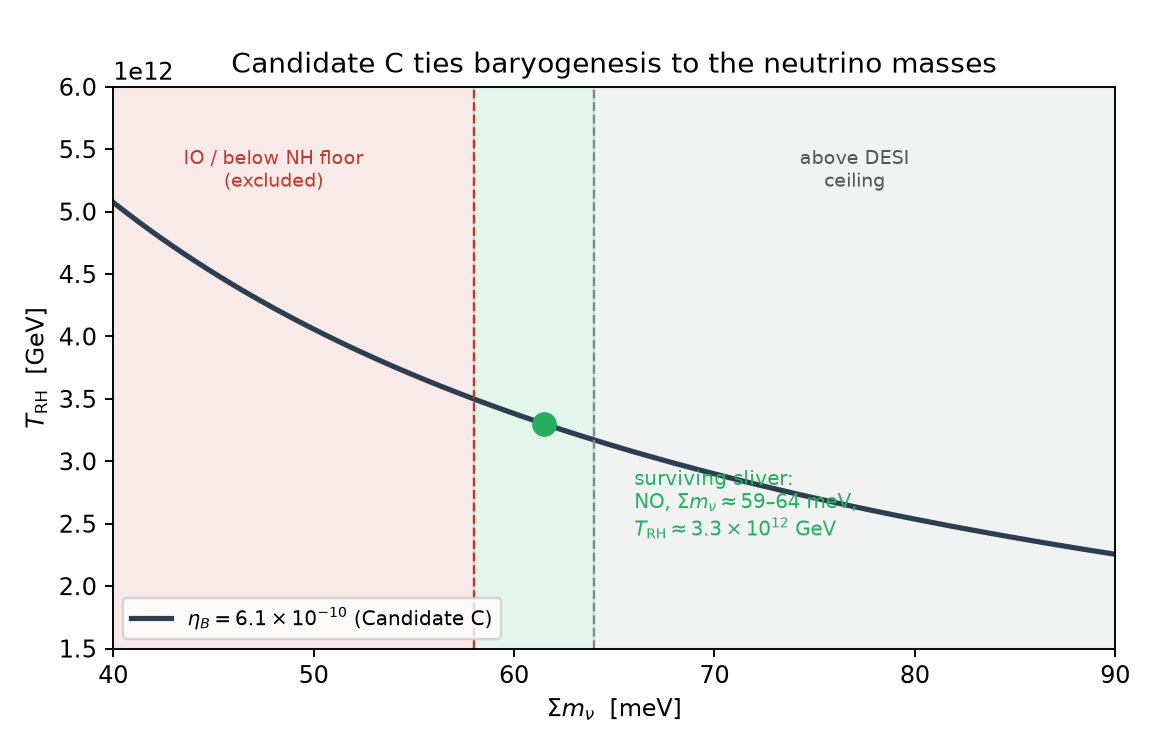
\includegraphics[keepaspectratio]{figures/fig2_candidateC.png}}
\caption{The Candidate-C squeeze. With
\(\eta_B\propto T_{\rm RH}^2(\Sigma m_\nu)^2\) fixed to the observed
\(6.1\times10^{-10}\), the normal-ordering floor and the DESI ceiling
bracket a thin surviving region: normal ordering,
\(\Sigma m_\nu\approx59\)--\(64\) meV,
\(T_{\rm RH}\approx3.3\times10^{12}\) GeV. Inverted ordering is
excluded; a DESI tightening below the NH floor kills the
variant.}\label{fig:2}
\end{figure}

Given the shared asymmetry and the sphaleron transfer, the dark-matter
mass is fixed by requiring the \emph{same} asymmetry to yield the
observed \(\Omega_{\rm DM}/\Omega_b\):

\begin{quote}
\(m_X = (\Omega_X/\Omega_b) \cdot m_p \cdot (28/79) / r_{X,BL} \approx 1.78\)
GeV at \(r_{X,BL} = 1\) (matched to \(\Omega_{\rm DM}/\Omega_b = 5.36\),
not predicted) \citep{Kaplan:2009ag}.
\end{quote}

This is \emph{matched}, not predicted:
\(\Omega_{\rm DM}/\Omega_b = 5.36\) is adopted from observation and
inverted for the mass. The flavored-charge ratio \(r_{X,BL}\) is a
genuine model uncertainty --- \(r_{X,BL} = 1\) gives 1.78 GeV, while the
older flavored correction gave \textasciitilde1.3 GeV
(\texttt{CONVENTIONS\_\allowbreak AND\_\allowbreak CORRECTIONS.\allowbreak md}). We adopt
\(m_X \approx 1.78\) GeV as the benchmark, with the honest note that an
earlier momentum-resolved-transport calculation finds \(m_X\) set by
\emph{sphaleron timing} (not washout),
\(m_X = 1.782 \cdot f_{\rm sph}(T_{\rm dec})\), landing at 1.78 GeV in
\textasciitilde89\% of its viable window
(\texttt{CONSOLIDATED\_\allowbreak THEORY.\allowbreak md}) --- a preliminary narrowing (single
volume/one-loop, not yet converged) that supports, but does not replace,
the matched normalization.

The dark matter is cold, asymmetric, and phenomenologically
near-invisible: \(\sigma_{\rm SI} \sim 2\times10^{-48}\) cm\(^{2}\),
below the neutrino fog. Its most distinctive external signature is
\emph{the absence of signatures} --- no direct detection, and (in horn
(i)) \(r \approx 0\) in primordial tensors.

We treat the dark-matter identity as a \textbf{three-horn} structure and
present all three honestly:

\textbf{Horn (i) --- pure ADM (ECCG-res-iv).} The condensate impulse
sources both sectors; \(\Omega_{\rm DM}/\Omega_b \approx 5\) is
\emph{explained} by the shared asymmetry, and \(m_X = 1.78\) GeV is
sharp. \(\eta_B\) is a fit (§\ref{sec-5-4}). Tensors:
\(r \leq 2\times10^{-11}\). This is the horn in which co-genesis does
its signature work --- the \(\Omega_{\rm DM}/\Omega_b\) coincidence is a
consequence, not an input. Its cost is that \(\eta_B\)'s magnitude is
not derived.

\textbf{Horn (ii) --- Candidate-C hybrid.} The clock+Weinberg channel
makes \(\eta_B\) calculable (§\ref{sec-5}) at the cost of discarding the
condensate, so \(m_X\) becomes a band (0.18--840 GeV) rather than a
sharp value, and the \(\Omega_{\rm DM}/\Omega_b\) coincidence is one
equation in two unknowns. This is the horn that ties \(\eta_B\) to the
neutrino sector --- a near-floor consistency constraint, not a
discriminating prediction (§\ref{sec-5}).

\textbf{Horn (iii) --- glueball one-sector.} The same hidden confining
sector that generates the \(\mu\) scale {[}Paper VI / scale sector{]}
supplies \(\Omega_{\rm DM}\) via 3→2 (SIMP/cannibal) glueball
freeze-out, with a \emph{predicted} mass
\(m_G = 6\Lambda_h = 180\text{–}630\) MeV (calculated across the
two-loop \(\Lambda_h = 28\text{–}105\) MeV band). Honest ledger entry
(\texttt{GLUEBALL\_\allowbreak DM\_\allowbreak assessment.\allowbreak md}): the SIMP ``miracle'' here is a
\textbf{mass} miracle (\(m_G\) lands where 3→2 works with a natural
coupling \(\alpha_{\rm eff} \approx 0.25\text{–}0.6\)), \textbf{not an
abundance miracle}. Pure glue has no renormalizable portal, so the
abundance is set by the hidden-to-visible temperature ratio \(\xi\), and
requires an inflaton branching
\(\mathrm{Br} \approx (0.4\text{–}3)\times10^{-10}\) selected to
\textasciitilde40\% --- a dial that \emph{replaces} ADM's explained
\(\Omega_{\rm DM}/\Omega_b\). This horn uniquely evades the
single-source theorem (§\ref{sec-10-1}) because glueball DM is
\emph{thermally} sourced, not clock-sourced, so it achieves both a
derived \(\eta_B\) (via Candidate C) and a predicted \(m_G\) --- at the
stated cost of the \(\mathrm{Br}\) dial. Its distinctive signature is
velocity-\emph{independent} self-interaction
\(\sigma/m \approx 0.01\text{–}0.47\) cm\(^{2}\)/g, already at the
cluster-constraint boundary for \(\Lambda_h \approx 30\) MeV.

\textbf{The environmental sign bit.} In all horns the \emph{magnitude}
\(|\eta_B|\) is predicted but the \emph{sign} is environmental:
spontaneous CP violation chooses between \(\pm\theta_S^{*}\) (exactly
degenerate CP partners), and inflation makes that choice uniform across
the observable universe. So the theory predicts that we live in a
matter-dominated (not antimatter-dominated) universe with the observed
magnitude, but does not predict \emph{which} --- a standard feature of
spontaneous-CPV baryogenesis, stated for honesty.

\begin{center}\rule{0.5\linewidth}{0.5pt}\end{center}

\section{Candidate C and neutrinos (D-2)}\label{sec-5}

\subsection{The channel}\label{sec-5-1}

Candidate C is the clock-driven variant in which baryogenesis proceeds
through the Weinberg operator (whose coefficient \emph{is} the neutrino
mass) \citep{Davidson:2008bu}, giving

\begin{quote}
\(\eta_B \propto T_{\rm RH}^{2} \cdot (\Sigma m_i^{2})\), more precisely
\(\eta_B \propto T_{\rm RH}^{2}\, \Sigma m_\nu^{2} / 2\pi\) (calculated
within the matched EFT).
\end{quote}

The washout mass is \(\bar{m}^{2} = \Sigma m_i^{2}\) (sum of
\emph{squares}), while cosmology bounds \(\Sigma m_i\) (sum) ---
different observables. D-2 maps between them via the lightest-mass
parametrization for NO and IO, using a real \(\Delta L=2\) washout
Boltzmann rather than the weak-washout analytic (which overshoots
13--31\% in-window). The calibration:
\(Y_B(3.17\times10^{12}, \text{NO-floor}) = 7.98\times10^{-11}\),
matching the shipped script.

\subsection{The squeeze}\label{sec-5-2}

Setting \(\eta_B = 6.10\times10^{-10}\) fixes the line
\(\eta_B \propto T_{\rm RH}^{2}\, \Sigma m_i^{2}\). Intersecting it with
the neutrino mass floors, the DESI ceiling, and ECCG's reheating window
gives a \textbf{razor-thin allowed region} (calculated, D-2):

\begin{quote}
\textbf{\(T_{\rm RH} \approx 3.28\text{–}3.31\times10^{12}\) GeV,
\(\Sigma m_\nu \approx 59\text{–}64\) meV, NORMAL ORDERING} (width in
\(T_{\rm RH}\): factor 1.01).
\end{quote}

The NO mass floor (58.6 meV) is matched at
\(T_{\rm RH} = 3.31\times10^{12}\) GeV; the DESI DR2 baseline ceiling
(64 meV) \citep{Elbers:2025vlz} is hit at
\(T_{\rm RH} = 3.28\times10^{12}\) GeV. The band is \(\leq 6\) meV wide
and sits exactly at the current DESI cut. The rest of the reheating
window (\(T_{\rm RH} \gtrsim 3.6\times10^{12}\) GeV) needs
\(\Sigma m_i^{2} <\) the NO floor --- impossible for any real neutrino
spectrum --- so it \emph{overproduces} \(\eta_B\). This is why D-1's
widening of the upper window edge (from \(\Lambda_H\) to the
portal-thermal \(9\times10^{12}\) GeV) does not change the result: the
extra room is all overproducing space; the viable sliver at
\(T_{\rm RH} \approx 3.3\times10^{12}\) GeV stands.

\subsection{The two sharp falsifiers, and the \textasciitilde1\%
survival}\label{sec-5-3}

\begin{itemize}
\tightlist
\item
  \textbf{Inverted ordering is excluded.} The IO floor
  (\(\Sigma m_\nu = 99\) meV) requires \(T_{\rm RH} = 2.4\times10^{12}\)
  GeV (below the reheating window) and lies far above the DESI ceiling
  \citep{Elbers:2025vlz, Hannestad:2016fog}. A confirmed IO kills
  Candidate C.
\item
  \textbf{DESI's aggressive bound is already below the NO floor.} The
  DESI DR2 + DESY5 combination gives \(\Sigma m_\nu < 46\) meV
  \citep{Elbers:2025vlz}, \emph{below} the 58.6 meV oscillation floor
  --- the emerging ``neutrino mass anomaly.'' If it holds, the Weinberg
  operator loses its anchor and Candidate C is falsified together with
  the mass floor itself.
\end{itemize}

Honestly, this is a \textbf{squeeze, not a parameter-free prediction}.
The O(1)-coupling systematic (\(g_\chi\), the Weinberg normalization
\(C_W\), \(g_*\)) is \(\approx  \times 13\) in \(T_{\rm RH}\); the
robustness scan finds that \emph{almost every point in that space is
already in tension} (raising \(g_\chi\) overproduces \(\eta_B\);
lowering \(C_W\) needs DESI-excluded 100--250 meV neutrinos). Only the
canonical point threads the window and a DESI-allowed NO mass ---
roughly \textasciitilde1\% of prior volume survives. The robust
statement is therefore \emph{not} ``C predicts \(\Sigma m_\nu = 60\)
meV'' but ``C's viable region is squeezed to NO + \(\Sigma m_\nu\) at
its floor + \(T_{\rm RH}\) at the bottom of the window, exactly where
DESI is cutting.'' The DESI numbers quoted (baseline 64 meV, aggressive
46 meV) \citep{Elbers:2025vlz} are representative as of early 2026 and
should be refreshed against the live posterior before quoting; the
\emph{structure} (floor-vs-ceiling squeeze) is robust to the exact
ceiling.

\subsection{\texorpdfstring{\(\eta_B\) is matched, not
four-times-derived}{ is matched, not four-times-derived}}\label{sec-5-4}

We are explicit about a meta-pattern the audit flagged (P3). The ECCG
corpus contains four ``independent confirmations'' of \(\eta_B\) ---
from \(\Delta_{\rm CP}\), \(m_3/H\), \(\eta_2\), and \(v_w\) --- but
each of these is computed through a \textbf{common calibrated
\texttt{predict\_\allowbreak eta\_\allowbreak B.\allowbreak py}} that already encodes the \(\eta_B\) fit;
each report tunes its own knob (\(\eta_3 = 1\), \(m_3/H\) solved,
bracket \(= 1\), \(T_*\) free) to reproduce the same
\(\eta_B \approx 6\times10^{-10}\). So ``four confirmations landing on
\(\eta_B\)'' is largely \textbf{one fit viewed four ways}. The magnitude
of \(\eta_B\) (equivalently \(m_3/H\)) is irreducibly a fit: an attempt
to derive it from maximum-entropy production overshoots by
\textasciitilde{}\(10^{9}\) (\texttt{USC\_\allowbreak m3\_\allowbreak derivation.\allowbreak md}). In
fairness, the natural (untuned) forward value is not absurd --- the
spontaneous-CP scan puts the \emph{median}
\(\eta_B = 1.21\times10^{-9}\) (16--84\% \([0.87, 1.47]\times10^{-9}\)),
so the observed \(6.1\times10^{-10}\) sits at roughly the
\textasciitilde29th--38th percentile of the natural distribution rather
than at a tuned edge. That is a genuine ``not fine-tuned to O(1)''
statement; it is \emph{not} a derivation of the magnitude, and \(m_3/H\)
is still solved to hit \(\eta_B\). We therefore present
\(\eta_B = 6.1\times10^{-10}\) as \textbf{matched, not predicted} (with
the rider that the natural value is within \textasciitilde×2), and the
dawn cross-checks as \emph{one consistency, not four predictions}. What
is \emph{not} a fit is the neutrino squeeze of §\ref{sec-5-2}, which
follows once the fitted \(\eta_B\) is combined with the \emph{measured}
\(\Sigma m_\nu^{2}\) and the reheating window --- that is the genuine
content of Candidate C.

\begin{center}\rule{0.5\linewidth}{0.5pt}\end{center}

\section{Honest status of the load-bearing strong-coupling
inputs}\label{sec-6}

The mechanism rests on three strong-coupling inputs that cannot be
closed at desk scale. Their honest status is the single most
over-claimed thing in prior program-level summaries, and we correct it
here. Each is now a fully-specified external project with a decision
rule (\texttt{EXTERNAL\_\allowbreak CALC\_\allowbreak SPECS.\allowbreak md}, items S-1/S-2/S-3).

\textbf{6.1 The first-order transition (S-1).} The 4D one-loop and 3D
dimensional-reduction legs are robust and give \(S_3/T_n = 52.3\),
\(\beta/H = 347\), \(\alpha = 0.027\) at
\(T_n \approx 3.2\times10^{12}\) GeV (calculated, within the matched
EFT). The \emph{lattice} leg is a \textbf{VALIDATED PIPELINE} (agreeing
at \(1.3\sigma\) with one published KKLP point,
\(\beta_{Hc} = 0.340879(7)\) vs digitized \(0.340868(5)\)) producing a
\textbf{PRELIMINARY} ECCG number at \emph{one volume
\((8^{2}\times 40)\), one spacing}, with one input digitized from a
figure. At the ECCG point the pipeline shows a clean double-peak
\(R^{2}\) histogram (a qualitative first-order signal) and
\(\beta_{Hc} = 0.344137(9)\), \(y3_c = 0.215 \pm 0.003\) (stat) --- but
with \textbf{no \(V \to \infty\) or \(a \to 0\) extrapolation}, and a
±0.03 dimensional-reduction systematic that dominates the statistical
error. The double-peak character is a robust qualitative result; the
\emph{number} is explicitly not a converged critical point. We therefore
write ``4D one-loop + 3D DR robust; lattice pipeline validated, ECCG
point preliminary --- continuum / infinite-volume convergence open.'' We
do \textbf{not} write ``first-order confirmed by lattice''; that is an
overclaim. The S-1 spec (9 volume/spacing combinations, susceptibility
scaling \(\propto V\) for first-order vs saturation for crossover,
\textasciitilde{}\(10^{6}\) core-hours) has an explicit decision rule:
\textbf{a crossover verdict at any spacing falsifies the mechanism as
constructed}, because it removes the out-of-equilibrium leg
(§\ref{sec-9}, F4).

\textbf{6.2 The SQCD confining vacuum (S-2).} The absolute scales of the
matter sector --- \(\Lambda_H\), \(\langle\Theta\rangle\), \(\kappa_2\)
--- come from a \textbf{one-loop qualitative} estimate at strong
coupling (\(g_H \approx 1.95\)). This is a benchmark-level qualitative
estimate, not a controlled value (preliminary and qualitative --- not
yet converged). The quantum-modified moduli constraint with positive
soft masses selects the diagonal branch \(|M_{ii}| = \Lambda_H^{2}\),
hence \(\arg\langle\Theta\rangle = 0\) --- a \emph{structural}, assumed
input to the D-1 domain cure (§\ref{sec-2-3}). S-2's decision rule
matters downstream: if the honest band on \(\langle\Theta\rangle\) moves
the derived \(\eta_B\) by more than the reheating-window width, the
Candidate-C neutrino squeeze shifts and must be re-quoted; the falsifier
currently carries this uncertainty silently.

\textbf{6.3 The wall velocity (S-3).} \(v_w = 0.58\) is a
\textbf{leading-order ballistic} friction estimate (near-sonic
deflagration/hybrid; the \(\pm0.09\) is an assumed NLO envelope, not
computed) --- preliminary and leading-order, not yet converged. At LO
the runaway check passes with margin ×2.40
(\(\Delta V(T_n) = 0.642\, T^{4}\) vs max net friction
\(1.540\, T^{4}\)), and the older benchmark \(v_w = 0.30\) is excluded
at LO. The paper's \(\eta_B\) uses \(v_w = 0.58\) as if converged; it is
not. The S-3 decision rule: \(v_w \in [0.3, 0.7]\) keeps \(\eta_B\)
stable within \textasciitilde×2 (claim survives); \(v_w \to 1\)
(runaway) drops the sourced asymmetry sharply and forces a re-fit of
\(m_3/H\) (a fine-tuning flag); \(v_w < 0.1\) tightens the DESI
\(\Sigma m_\nu\) squeeze.

\begin{center}\rule{0.5\linewidth}{0.5pt}\end{center}

\section{The revised benchmark under the resolution}\label{sec-7}

For the record, several quantities shifted under the resolution that
produced the current benchmark, and un-updated corpus documents may
still carry the old values (a bookkeeping caveat, not a physics change):
\(m_X: 1.30 \to 1.78\) GeV; \(f_B: 0.259 \to 28/79 = 0.354\);
\(m_3/H: 1.84 \to 1.58\); \(v_w: 0.30 \to 0.58\) (estimated). We quote
the resolved values throughout.

\begin{center}\rule{0.5\linewidth}{0.5pt}\end{center}

\section{\texorpdfstring{The gauged-CP \(\mathrm{Pin}^+\)
\(\nu \bmod 16\) anomaly}{The gauged-CP   anomaly}}\label{sec-8}

Gauging CP (making the spontaneous-CP construction consistent as a gauge
theory in 3+1d with \(\mathrm{Pin}^+\) structure) carries a
\(\mathbb{Z}_{16}\)-valued Dai--Freed anomaly
(\(\Omega^{\mathrm{Pin}^+}_5 \supset \mathbb{Z}_{16}\);
Fidkowski--Kitaev, Witten): each Majorana fermion contributes
\(\nu = \pm1 \bmod 16\), and consistency requires the total
\(\nu = 0 \bmod 16\). We \textbf{exhibit an explicit satisfying
assignment} (an explicit construction, weaker than a derivation): the
\textasciitilde16 CP-relevant Weyl fermions of the R3 realization pair
up under the report's own massability structure (four R3 spectator
pairs, the condensate-ino conjugate pairs, the \(\mathbb{Z}_{31}\)
spectators), each pair carrying opposite intrinsic CP phases
\((+1, -1)\) and contributing 0, for a total \(\nu = 0 \bmod 16\)
(\texttt{PIN16\_\allowbreak assignment\_\allowbreak constructed.\allowbreak md},
\texttt{S3\_\allowbreak GAUGING\_\allowbreak REPORT}). This is \emph{stronger than
``satisfiable''} --- the per-pair sign flip never changes the sum, so
\(\nu = 0\) is automatic given CP-commuting mass dressings, and each
pair has its own spurion channel so the phases are absorbable one pair
at a time. But we say plainly: \textbf{this is a construction, not a
derivation.} It shows a consistent assignment exists; it does not show
one is forced, and a future enlargement of the chiral content re-opens
the count.

\begin{center}\rule{0.5\linewidth}{0.5pt}\end{center}

\section{Falsifiers}\label{sec-9}

The dawn face is over-determined by several handles that are
\emph{observationally independent} of one another and of the rest of the
program. We number the falsifiers; each maps to a pre-registered entry
(Zenodo \texttt{10.\allowbreak 5281/\allowbreak zenodo.\allowbreak 21415326}).

\begin{itemize}
\tightlist
\item
  \textbf{F1 --- DESI \(\Sigma m_\nu\).} If DESI DR2/DR3 tightens
  \(\Sigma m_\nu\) below the \textasciitilde59 meV NO floor
  \citep{Elbers:2025vlz}, Candidate C (horns ii, iii) is falsified. This
  is the union's most imminent make-or-break test; the current baseline
  (64 meV) already sits at the top of the allowed sliver, and the
  aggressive combination (46 meV) is already below the floor.
\item
  \textbf{F2 --- Inverted ordering.} A confirmed IO neutrino spectrum
  kills Candidate C outright (§\ref{sec-5-3}).
\item
  \textbf{F3 --- Neutron EDM (branch B).} The D-1 cure forces
  \(T_{\rm RH} < v_S\); the economical branch-B flavon
  (\(v_S = 2.44\times10^{13}\) GeV) sits at the nEDM edge,
  \(\bar{\theta} \sim (v_S/M_{\rm Pl})^{2} \sin\Delta_{\rm CP} \sim 4\times10^{-12}\cdot\mathrm{O}(1)\),
  predicting a neutron EDM near \(\sim10^{-27}\) \(e\cdot cm\) --- a
  DESI/CMB-independent handle. (Branch A evades nEDM but requires a
  second gauged flavon.) A null result at improved sensitivity disfavors
  branch B; a detection at the bound supports horn (i).
\item
  \textbf{F4 --- The lattice first-order verdict (S-1).} If a converged
  lattice run finds the transition is a \textbf{crossover} at any
  spacing, the out-of-equilibrium Sakharov leg is gone and the mechanism
  as constructed is falsified (§6.1).
\item
  \textbf{F5 --- Wall-velocity runaway (S-3).} If the full transport
  solve gives \(v_w \to 1\) (runaway), the sourced asymmetry drops
  sharply, breaking the ``no fine-tuning'' claim and forcing a re-fit of
  \(m_3/H\) (§6.3).
\item
  \textbf{F6 --- Primordial tensors (horn selector).} Horn (i) predicts
  \(r \leq 2\times10^{-11}\) (\(r \approx 0\)); \emph{any} tensor
  detection kills horn (i) and selects the Candidate-C horns (ii/iii),
  which allow \(r\). This is the tensor split of the two-horn theorem,
  cross-linked to the galactic face (a rising \(a_0(z)\) \(\iff\)
  \(r \approx 0\) \(\iff\) 1.78 GeV DM).
\end{itemize}

\begin{center}\rule{0.5\linewidth}{0.5pt}\end{center}

\section{Relation to the program}\label{sec-10}

\subsection{The single-source theorem and the two-horn
structure}\label{sec-10-1}

The dawn is a \textbf{two-horn theorem}, and the reason is a genuine,
calculated EFT result:

\begin{quote}
\textbf{Generalized single-source theorem.} In any clock-driven
co-genesis, the chemical potential \(\mu = H/2\pi\) cancels in the ratio
\(Y_X/Y_B\). Hence \textbf{\(\eta_B\)-calculable and \(m_X\)-sharp are
mutually exclusive.}
\end{quote}

Horn (i) (ECCG-res-iv) keeps \(m_X = 1.78\) GeV sharp at the cost of
\(\eta_B\) being a fit; horn (ii) (Candidate C) makes \(\eta_B\)
calculable (because \(\Sigma m_\nu^{2}\) is \emph{measured}) at the cost
of \(m_X\) becoming a band. The two horns are split observationally by
primordial tensors (F6). Horn (iii) (glueball) \emph{evades} the theorem
because glueball DM is thermally sourced, not clock-sourced --- the
premise (\(\mu = H/2\pi\) in both yields) fails --- so it uniquely gets
both a derived \(\eta_B\) and a predicted \(m_G\), relocating the
theorem's content from the DM mass to the DM abundance (the
\(\mathrm{Br}\) dial). The theorem's content is conserved, not evaded.

\subsection{\texorpdfstring{The clock does not source matter
(\(R_0 = 0\))}{The clock does not source matter ()}}\label{sec-10-2}

We restate the negative result of §\ref{sec-1-1} because it is
structurally important to the unification: the entropy clock
\(\mathcal{D}_E = (3/2)(1-w)\) links the \emph{timing} and
\emph{thermodynamics} of the three faces, but it does \textbf{not}
source the matter asymmetry. The candidate direct-source operator is
\(\mathbb{Z}_2\)-even, so \(R_0 = 0\) by symmetry (a calculated symmetry
theorem). This is what makes ECCG a pre-inflationary initial-condition
theory rather than a clock-pumped one, and it is why the program's
honesty survives: the clock's unifying role is real (it is the same
variable that reads \(\mathcal{D}_E \to 3\) at dusk and sets
\(a_0 \propto (3/2)(1+w)\) galactically) without over-claiming a matter
source it does not have.

\subsection{Connection to dusk and the scale sector}\label{sec-10-3}

Two threads connect this paper outward. \textbf{To dusk (SEDE):} ECCG's
\textasciitilde1.78 GeV ADM \emph{is} SEDE's assumed cold dark matter,
whose collapse drives the growth gate of the dark-energy model {[}Paper
III / SEDE cosmology{]}, and the identity \(\omega_b \equiv \eta_B\)
removes SEDE's baryon-density fit --- so the union is more falsifiable
than \(\Lambda \mathrm{CDM}\) at equal continuous-parameter count.
\textbf{To the scale sector:} horn (iii)'s glueball mass
\(m_G = 6\Lambda_h\) and (via the transmutation identity) the MOND scale
\(a_0\) are set by the same \(\Lambda_h\) that fixes the \(\mu\) scale
{[}Paper VI / scale sector{]}, through the chain
\(\alpha_s(M_{\rm Pl}) \to \Lambda_h \to \mu \to a_0\). The dawn is thus
the hinge of the program: it delivers the matter that dusk assumes and
shares the confining scale that the galactic face reads.

\begin{center}\rule{0.5\linewidth}{0.5pt}\end{center}

\section{Discussion and limitations}\label{sec-11}

ECCG is, honestly, a \textbf{matched-EFT existence proof} of GeV-scale
asymmetric co-genesis, not a fully predictive theory. Its strengths are
real: one genuinely-calculated closure (\(f_B = 28/79\)), a
self-consistent pre-inflationary history that survives reheating (D-1),
a near-floor neutrino consistency constraint (Candidate C → NO,
\(\Sigma m_\nu \approx 59\text{–}64\) meV), and a clean
over-determination against the rest of the program. Its limitations are
equally real and we do not hide them:

\begin{enumerate}
\def\labelenumi{\arabic{enumi}.}
\tightlist
\item
  \textbf{The sign is environmental} --- the magnitude of \(\eta_B\) is
  predicted, the sign is not (spontaneous CPV).
\item
  \textbf{The magnitude of \(\eta_B\) is a fit} --- \(m_3/H\) is fitted,
  MaxEP fails by \textasciitilde{}\(10^{9}\), and the ``four
  confirmations'' share one calibrated normalization (§\ref{sec-5-4}).
\item
  \textbf{The microscopic sector is benchmark/qualitative/preliminary}
  --- first-order transition (lattice preliminary), SQCD vacuum
  (one-loop qualitative), \(v_w\) (LO ballistic). These are validated
  pipelines and specified projects, not confirmed results.
\item
  \textbf{The \(\mathrm{Pin}^+\) anomaly cancellation is constructed,
  not derived} (§\ref{sec-8}).
\item
  \textbf{\(m_X\)'s exact value depends on \(r_{X,BL}\)} (1.78 GeV at
  \(r_{X,BL}=1\)), and horns (ii)/(iii) trade the sharp mass for a band
  or a \(\mathrm{Br}\) dial.
\end{enumerate}

The correct summary is not ``the dawn is calculated'' but ``the dawn is
a coherent, over-determined, imminently falsifiable existence proof with
one calculated closure, whose remaining ignorance is either irreducibly
a fit (\(\eta_B\) magnitude, the sign) or purchasable with compute
(S-1/S-2/S-3).''

\begin{center}\rule{0.5\linewidth}{0.5pt}\end{center}

\section{Reproducibility}\label{sec-12}

The results above reproduce from the accompanying analysis scripts in
\url{https://github.com/spsingularity/eccg-matter-genesis} (a tagged
release is archived at Zenodo, DOI 10.5281/zenodo.21525535). Key scripts
and reports:

\begin{itemize}
\tightlist
\item
  \textbf{Sphaleron / \(f_B\):}
  \texttt{CLOSURES\_\allowbreak assumed\_\allowbreak vs\_\allowbreak calculated.\allowbreak md} (N4); Harvey--Turner
  counting.
\item
  \textbf{Spontaneous CP / \(\Delta_{\rm CP}\):}
  \texttt{spontaneous\_\allowbreak cp.\allowbreak py} → \texttt{SPONTANEOUS\_\allowbreak CP\_\allowbreak REPORT.\allowbreak md}
  (scan, \texttt{spontaneous\_\allowbreak cp\_\allowbreak scan.\allowbreak csv}, 40,000 draws).
\item
  \textbf{Pre-inflation reheating cure (D-1):}
  \texttt{sims/\allowbreak preinflation\_\allowbreak reheat\_\allowbreak domain\_\allowbreak check.\allowbreak py} →
  \texttt{D1\_\allowbreak result\_\allowbreak preinflation\_\allowbreak reheating.\allowbreak md}.
\item
  \textbf{Candidate C neutrino inversion (D-2):}
  \texttt{sims/\allowbreak candidateC\_\allowbreak neutrino\_\allowbreak inversion.\allowbreak py},
  \texttt{candidateC\_\allowbreak yield.\allowbreak py} →
  \texttt{D2\_\allowbreak result\_\allowbreak candidateC\_\allowbreak neutrino.\allowbreak md}; figure
  \texttt{figures/\allowbreak candidateC\_\allowbreak neutrino\_\allowbreak inversion.\allowbreak png}.
\item
  \textbf{Wall velocity (S-3):} \texttt{wall\_\allowbreak velocity\_\allowbreak precise.\allowbreak py} →
  \texttt{WALL\_\allowbreak VELOCITY\_\allowbreak PRECISE\_\allowbreak REPORT.\allowbreak md}.
\item
  \textbf{Global scan / benchmark point:}
  \texttt{GLOBAL\_\allowbreak SCAN\_\allowbreak REPORT.\allowbreak md}.
\item
  \textbf{Flavor / \(S_3\) gauging / \(\mathrm{Pin}^+\)
  \(\nu \bmod 16\):} \texttt{FLAVOR\_\allowbreak MODEL\_\allowbreak REPORT.\allowbreak md},
  \texttt{S3\_\allowbreak GAUGING\_\allowbreak REPORT.\allowbreak md},
  \texttt{PIN16\_\allowbreak assignment\_\allowbreak constructed.\allowbreak md}.
\item
  \textbf{Glueball DM horn:} \texttt{sims/\allowbreak glueball\_\allowbreak simp\_\allowbreak relic.\allowbreak py} →
  \texttt{GLUEBALL\_\allowbreak DM\_\allowbreak assessment.\allowbreak md}.
\item
  \textbf{External calculation specs (S-1/S-2/S-3):}
  \texttt{EXTERNAL\_\allowbreak CALC\_\allowbreak SPECS.\allowbreak md} (decision rules).
\item
  \textbf{\(\eta_B\) provenance / P3 meta-pattern:}
  \texttt{predict\_\allowbreak eta\_\allowbreak B.\allowbreak py}; \texttt{AUDIT\_\allowbreak round2\_\allowbreak sweep.\allowbreak md},
  \texttt{CLOSURES\_\allowbreak assumed\_\allowbreak vs\_\allowbreak calculated.\allowbreak md}.
\item
  \textbf{Pre-registration:}
  \texttt{PREREGISTRATION\_\allowbreak falsifier\_\allowbreak matrix.\allowbreak md} (Zenodo
  \texttt{10.\allowbreak 5281/\allowbreak zenodo.\allowbreak 21415326}).
\end{itemize}

Companion papers: {[}Paper III / SEDE cosmology, Zenodo
10.5281/zenodo.21525525{]}, {[}Paper V / USC framework, Zenodo
10.5281/zenodo.21525529{]}, {[}Paper VI / scale sector, Zenodo
10.5281/zenodo.21525533{]}, {[}Paper VIII / APDM galactic, Zenodo
10.5281/zenodo.21525537{]}.

\begin{center}\rule{0.5\linewidth}{0.5pt}\end{center}

\section*{Acknowledgements}\label{acknowledgements}
\addcontentsline{toc}{section}{Acknowledgements}

We thank the ECCG development team whose gap-closure reports (with their
explicit VALIDATED / PRELIMINARY / DIGITIZED / QUALITATIVE tags) set the
audit culture this paper inherits; carrying those tags upward is the
central discipline of this manuscript.

\textbf{AI assistance:} the analysis and drafting of this paper were
carried out with the assistance of Claude (Anthropic); all claims were
verified against the corpus's reproducing scripts and reports.

\begin{center}\rule{0.5\linewidth}{0.5pt}\end{center}

\bibliographystyle{apsrev4-2}
\bibliography{refs}
\end{document}
